%%
%% Automatically generated file from DocOnce source
%% (https://github.com/hplgit/doconce/)
%%

% #define PREAMBLE

% #ifdef PREAMBLE
%-------------------- begin preamble ----------------------

\documentclass[%
oneside,                 % oneside: electronic viewing, twoside: printing
final,                   % draft: marks overfull hboxes, figures with paths
10pt,french]{article}

\listfiles               %  print all files needed to compile this document

\usepackage{relsize,makeidx,color,setspace,amsmath,amsfonts,amssymb}
\usepackage[table]{xcolor}
\usepackage{bm,ltablex,microtype}

\usepackage[pdftex]{graphicx}

% Packages for typesetting blocks of computer code
\usepackage{fancyvrb,framed,moreverb}

% Define colors
\definecolor{orange}{cmyk}{0,0.4,0.8,0.2}
\definecolor{tucorange}{rgb}{1.0,0.64,0}
\definecolor{darkorange}{rgb}{.71,0.21,0.01}
\definecolor{darkgreen}{rgb}{.12,.54,.11}
\definecolor{myteal}{rgb}{.26, .44, .56}
\definecolor{gray}{gray}{0.45}
\definecolor{mediumgray}{gray}{.8}
\definecolor{lightgray}{gray}{.95}
\definecolor{brown}{rgb}{0.54,0.27,0.07}
\definecolor{purple}{rgb}{0.5,0.0,0.5}
\definecolor{darkgray}{gray}{0.25}
\definecolor{darkblue}{rgb}{0,0.08,0.45}
\definecolor{darkblue2}{rgb}{0,0,0.8}
\definecolor{lightred}{rgb}{1.0,0.39,0.28}
\definecolor{lightgreen}{rgb}{0.48,0.99,0.0}
\definecolor{lightblue}{rgb}{0.53,0.81,0.92}
\definecolor{lightblue2}{rgb}{0.3,0.3,1.0}
\definecolor{lightpurple}{rgb}{0.87,0.63,0.87}
\definecolor{lightcyan}{rgb}{0.5,1.0,0.83}

\colorlet{comment_green}{green!50!black}
\colorlet{string_red}{red!60!black}
\colorlet{keyword_pink}{magenta!70!black}
\colorlet{indendifier_green}{green!70!white}

% Backgrounds for code
\definecolor{cbg_gray}{rgb}{.95, .95, .95}
\definecolor{bar_gray}{rgb}{.92, .92, .92}

\definecolor{cbg_yellowgray}{rgb}{.95, .95, .85}
\definecolor{bar_yellowgray}{rgb}{.95, .95, .65}

\colorlet{cbg_yellow2}{yellow!10}
\colorlet{bar_yellow2}{yellow!20}

\definecolor{cbg_yellow1}{rgb}{.98, .98, 0.8}
\definecolor{bar_yellow1}{rgb}{.98, .98, 0.4}

\definecolor{cbg_red1}{rgb}{1, 0.85, 0.85}
\definecolor{bar_red1}{rgb}{1, 0.75, 0.85}

\definecolor{cbg_blue1}{rgb}{0.87843, 0.95686, 1.0}
\definecolor{bar_blue1}{rgb}{0.7,     0.95686, 1}

%\setlength{\fboxsep}{-1.5mm}  % adjust cod_vpad/pro_vpad background box

%% Background for code blocks (parameter is color name)

%% pro/cod_vpad: gives some vertical padding before and after the text
%% (but has more simplistic code than _cod/pro_tight+cod/pro).
%% pro/cod_vpad can be used to enclose Verbatim or lst begin/end for code.
%% pro/cod calls _pro/cod_tight and has very little vertical padding,
%% used to enclose Verbatim and other begin/end for code.
%% (pro/cod is what the ptex2tex program could produce with the
%% Blue/BlueBar definitions in .ptex2tex.cfg.)

\newenvironment{cod_vpad}[1]{
   \def\FrameCommand{\colorbox{#1}}
   \MakeFramed{\FrameRestore}}
   {\endMakeFramed}

\newenvironment{_cod_tight}[1]{
   \def\FrameCommand{\colorbox{#1}}
   \FrameRule0.6pt\MakeFramed {\FrameRestore}\vskip3mm}
   {\vskip0mm\endMakeFramed}

\newenvironment{cod}[1]{
\bgroup\rmfamily
\fboxsep=0mm\relax
\begin{_cod_tight}{#1}
\list{}{\parsep=-2mm\parskip=0mm\topsep=0pt\leftmargin=2mm
\rightmargin=2\leftmargin\leftmargin=4pt\relax}
\item\relax}
{\endlist\end{_cod_tight}\egroup}

%% Background for complete program blocks (parameter 1 is color name
%% for background, parameter 2 is color for left bar)
\newenvironment{pro_vpad}[2]{
   \def\FrameCommand{\color{#2}\vrule width 1mm\normalcolor\colorbox{#1}}
   \MakeFramed{\FrameRestore}}
   {\endMakeFramed}

\newenvironment{_pro_tight}[2]{
   \def\FrameCommand{\color{#2}\vrule width 1mm\normalcolor\colorbox{#1}}
   \FrameRule0.6pt\MakeFramed {\advance\hsize-2mm\FrameRestore}\vskip3mm}
   {\vskip0mm\endMakeFramed}

\newenvironment{pro}[2]{
\bgroup\rmfamily
\fboxsep=0mm\relax
\begin{_pro_tight}{#1}{#2}
\list{}{\parsep=-2mm\parskip=0mm\topsep=0pt\leftmargin=2mm
\rightmargin=2\leftmargin\leftmargin=4pt\relax}
\item\relax}
{\endlist\end{_pro_tight}\egroup}

\usepackage{minted}
\usemintedstyle{default}

\usepackage[T1]{fontenc}
%\usepackage[latin1]{inputenc}
\usepackage{ucs}
\usepackage[utf8x]{inputenc}

\usepackage{lmodern}         % Latin Modern fonts derived from Computer Modern

% Hyperlinks in PDF:
\definecolor{linkcolor}{rgb}{0,0,0.4}
\usepackage{hyperref}
\hypersetup{
    breaklinks=true,
    colorlinks=true,
    linkcolor=linkcolor,
    urlcolor=linkcolor,
    citecolor=black,
    filecolor=black,
    %filecolor=blue,
    pdfmenubar=true,
    pdftoolbar=true,
    bookmarksdepth=3   % Uncomment (and tweak) for PDF bookmarks with more levels than the TOC
    }
%\hyperbaseurl{}   % hyperlinks are relative to this root

\setcounter{tocdepth}{2}  % levels in table of contents

% Tricks for having figures close to where they are defined:
% 1. define less restrictive rules for where to put figures
\setcounter{topnumber}{2}
\setcounter{bottomnumber}{2}
\setcounter{totalnumber}{4}
\renewcommand{\topfraction}{0.95}
\renewcommand{\bottomfraction}{0.95}
\renewcommand{\textfraction}{0}
\renewcommand{\floatpagefraction}{0.75}
% floatpagefraction must always be less than topfraction!
% 2. ensure all figures are flushed before next section
\usepackage[section]{placeins}
% 3. enable begin{figure}[H] (often leads to ugly pagebreaks)
%\usepackage{float}\restylefloat{figure}

% --- fancyhdr package for fancy headers ---
\usepackage{fancyhdr}
\fancyhf{} % sets both header and footer to nothing
\renewcommand{\headrulewidth}{0pt}
\fancyfoot[LE,RO]{\thepage}
% Ensure copyright on titlepage (article style) and chapter pages (book style)
\fancypagestyle{plain}{
  \fancyhf{}
  \fancyfoot[C]{{\footnotesize \copyright\ 2019, Ahmed Ammar. Released under CC Attribution 4.0 license}}
%  \renewcommand{\footrulewidth}{0mm}
  \renewcommand{\headrulewidth}{0mm}
}
% Ensure copyright on titlepages with \thispagestyle{empty}
\fancypagestyle{empty}{
  \fancyhf{}
  \fancyfoot[C]{{\footnotesize \copyright\ 2019, Ahmed Ammar. Released under CC Attribution 4.0 license}}
  \renewcommand{\footrulewidth}{0mm}
  \renewcommand{\headrulewidth}{0mm}
}

\pagestyle{fancy}


\usepackage{framed,wrapfig}

% --- begin definitions of admonition environments ---

% Admonition style "grayicon" has colored background, no frame, and an icon
% Admon "notice"
\definecolor{grayicon_notice_background}{rgb}{0.91,0.91,0.91}
% \fboxsep sets the space between the text and the box
\newenvironment{noticeshaded}
{\def\FrameCommand{\fboxsep=3mm\colorbox{grayicon_notice_background}}
 \MakeFramed {\advance\hsize-\width \FrameRestore}}{\endMakeFramed}

\newenvironment{notice_grayiconadmon}[1][À noter]{
\begin{noticeshaded}
\noindent
\begin{wrapfigure}{l}{0.07\textwidth}
\vspace{-13pt}

\includegraphics[width=0.07\textwidth]{latex_figs/small_gray_notice}
\end{wrapfigure} \textbf{#1}\par
\nobreak\noindent\ignorespaces
}
{
\end{noticeshaded}
}

% Admonition style "grayicon" has colored background, no frame, and an icon
% Admon "summary"
\definecolor{grayicon_summary_background}{rgb}{0.91,0.91,0.91}
% \fboxsep sets the space between the text and the box
\newenvironment{summaryshaded}
{\def\FrameCommand{\fboxsep=3mm\colorbox{grayicon_summary_background}}
 \MakeFramed {\advance\hsize-\width \FrameRestore}}{\endMakeFramed}

\newenvironment{summary_grayiconadmon}[1][Résumé]{
\begin{summaryshaded}
\noindent
\begin{wrapfigure}{l}{0.07\textwidth}
\vspace{-13pt}
\includegraphics[width=0.07\textwidth]{latex_figs/small_gray_summary}
\end{wrapfigure} \textbf{#1}\par
\nobreak\noindent\ignorespaces
}
{
\end{summaryshaded}
}

% Admonition style "grayicon" has colored background, no frame, and an icon
% Admon "warning"
\definecolor{grayicon_warning_background}{rgb}{0.91,0.91,0.91}
% \fboxsep sets the space between the text and the box
\newenvironment{warningshaded}
{\def\FrameCommand{\fboxsep=3mm\colorbox{grayicon_warning_background}}
 \MakeFramed {\advance\hsize-\width \FrameRestore}}{\endMakeFramed}

\newenvironment{warning_grayiconadmon}[1][Attention]{
\begin{warningshaded}
\noindent
\begin{wrapfigure}{l}{0.07\textwidth}
\vspace{-13pt}

\includegraphics[width=0.07\textwidth]{latex_figs/small_gray_warning}
\end{wrapfigure} \textbf{#1}\par
\nobreak\noindent\ignorespaces
}
{
\end{warningshaded}
}

% Admonition style "grayicon" has colored background, no frame, and an icon
% Admon "question"
\definecolor{grayicon_question_background}{rgb}{0.91,0.91,0.91}
% \fboxsep sets the space between the text and the box
\newenvironment{questionshaded}
{\def\FrameCommand{\fboxsep=3mm\colorbox{grayicon_question_background}}
 \MakeFramed {\advance\hsize-\width \FrameRestore}}{\endMakeFramed}

\newenvironment{question_grayiconadmon}[1][Question]{
\begin{questionshaded}
\noindent
\begin{wrapfigure}{l}{0.07\textwidth}
\vspace{-13pt}
\includegraphics[width=0.07\textwidth]{latex_figs/small_gray_question2}
\end{wrapfigure} \textbf{#1}\par
\nobreak\noindent\ignorespaces
}
{
\end{questionshaded}
}

% Admonition style "grayicon" has colored background, no frame, and an icon
% Admon "block"
\definecolor{grayicon_block_background}{rgb}{0.91,0.91,0.91}
% \fboxsep sets the space between the text and the box
\newenvironment{blockshaded}
{\def\FrameCommand{\fboxsep=3mm\colorbox{grayicon_block_background}}
 \MakeFramed {\advance\hsize-\width \FrameRestore}}{\endMakeFramed}

\newenvironment{block_grayiconadmon}[1][Block]{
\begin{blockshaded}
\noindent
 \textbf{#1}\par
\nobreak\noindent\ignorespaces
}
{
\end{blockshaded}
}

% --- end of definitions of admonition environments ---

% prevent orhpans and widows
\clubpenalty = 10000
\widowpenalty = 10000

\newenvironment{doconceexercise}{}{}
\newcounter{doconceexercisecounter}
% --- begin definition of \listofexercises command ---
\makeatletter
\newcommand\listofexercises{\section*{List of Exercises}
\@starttoc{loe}
}
\newcommand*{\l@doconceexercise}{\@dottedtocline{0}{0pt}{6.5em}}
\makeatother
% --- end definition of \listofexercises command ---



% ------ header in subexercises ------
%\newcommand{\subex}[1]{\paragraph{#1}}
%\newcommand{\subex}[1]{\par\vspace{1.7mm}\noindent{\bf #1}\ \ }
\makeatletter
% 1.5ex is the spacing above the header, 0.5em the spacing after subex title
\newcommand\subex{\@startsection{paragraph}{4}{\z@}%
                  {1.5ex\@plus1ex \@minus.2ex}%
                  {-0.5em}%
                  {\normalfont\normalsize\bfseries}}
\makeatother


% --- end of standard preamble for documents ---


\usepackage[french]{babel}

% insert custom LaTeX commands...

\raggedbottom
\makeindex
\usepackage[totoc]{idxlayout}   % for index in the toc
\usepackage[nottoc]{tocbibind}  % for references/bibliography in the toc

%-------------------- end preamble ----------------------

\begin{document}

% matching end for #ifdef PREAMBLE
% #endif

\newcommand{\exercisesection}[1]{\subsection*{#1}}


% ------------------- main content ----------------------



% ----------------- title -------------------------

\thispagestyle{empty}

\begin{center}
{\LARGE\bf
\begin{spacing}{1.25}
TD N°2 : Contrôle du flux d’instructions
\end{spacing}
}
\end{center}

% ----------------- author(s) -------------------------

\begin{center}
{\bf Ahmed Ammar (\texttt{ahmed.ammar@fst.utm.tn})}
\end{center}

    \begin{center}
% List of all institutions:
\centerline{{\small Institut Préparatoire aux Études Scientifiques et Techniques, Université de Carthage.}}
\end{center}
    
% ----------------- end author(s) -------------------------

% --- begin date ---
\begin{center}
Nov 6, 2019
\end{center}
% --- end date ---

\vspace{1cm}


\tableofcontents


\vspace{1cm} % after toc






% --- begin exercise ---
\begin{doconceexercise}
\refstepcounter{doconceexercisecounter}

\exercisesection{Exercise \thedoconceexercisecounter: Comparer deux entiers}


Écrivez un programme qui vous demande de saisir 2 nombres entiers et affiche la plus petite de ces valeurs.


% --- begin solution of exercise ---
\paragraph{Solution.}
\begin{cod}{cbg_gray}\begin{minted}[fontsize=\fontsize{9pt}{9pt},linenos=false,mathescape,baselinestretch=1.0,fontfamily=tt,xleftmargin=2mm]{python}
# %load solution/ex1
valeur1= int(input("Valeur 1 : "))
valeur2= int(input("Valeur 2 : "))
if (valeur1 < valeur2 ) :
    print("Valeur la plus petite : ", valeur1)
else:
    print("Valeur la plus petite : ", valeur2)
\end{minted}
\end{cod}
\noindent

% --- end solution of exercise ---

\end{doconceexercise}
% --- end exercise ---




% --- begin exercise ---
\begin{doconceexercise}
\refstepcounter{doconceexercisecounter}

\exercisesection{Exercise \thedoconceexercisecounter: Comparer deux chaînes}


Écrivez un programme qui demande d'entrer 2 chaînes et qui affiche la plus grande des 2 chaînes (celle qui contient le plus de caractères).


% --- begin solution of exercise ---
\paragraph{Solution.}
\begin{cod}{cbg_gray}\begin{minted}[fontsize=\fontsize{9pt}{9pt},linenos=false,mathescape,baselinestretch=1.0,fontfamily=tt,xleftmargin=2mm]{python}
# %load solution/ex2
chaine1= input("Chaîne 1 : ")
chaine2= input("Chaîne 2 : ")

if len(chaine2) > len(chaine1) :
    print ("Chaîne la plus grande : " , chaine2 )
else:
    print ("Chaîne la plus grande : " , chaine1 )
\end{minted}
\end{cod}
\noindent

% --- end solution of exercise ---

\end{doconceexercise}
% --- end exercise ---




% --- begin exercise ---
\begin{doconceexercise}
\refstepcounter{doconceexercisecounter}

\exercisesection{Exercise \thedoconceexercisecounter: Convertir Euro contre Dinar Tunisien | EUR TND}


Écrivez un programme qui convertit l'euro (EUR) en dinar tunisien (TND):

\begin{itemize}
\item Le programme commence par demander à l'utilisateur d'indiquer par une chaîne de caractères 'EUR' ou 'TND' la devise du montant qu'il entrera.

\item Ensuite, le programme exécute une action conditionnelle de la forme:
\end{itemize}

\noindent
\begin{cod}{cbg_gray}\begin{minted}[fontsize=\fontsize{9pt}{9pt},linenos=false,mathescape,baselinestretch=1.0,fontfamily=tt,xleftmargin=2mm]{python}
if devise == 'EUR' :
    # Expression 1
elif devise == 'TND' :
    # Expression 2
else :
   # affichage d'un message d'erreur
\end{minted}
\end{cod}
\noindent


% --- begin solution of exercise ---
\paragraph{Solution.}
\begin{cod}{cbg_gray}\begin{minted}[fontsize=\fontsize{9pt}{9pt},linenos=false,mathescape,baselinestretch=1.0,fontfamily=tt,xleftmargin=2mm]{python}
# %load solution/ex3
devise = input("Devise : ")
montant = int(input ("Montant : "))
# 1 EUR = 3.30 TND
facteur_euro_dinar = 3.30
if devise == 'EUR' :
    print ("{} TND".format(montant * facteur_euro_dinar))

elif devise == 'TND' :
    print ("{} Euros".format(montant / facteur_euro_dinar))

else :
    print ("Je n'ai rien compris") # affichage d'un message d'erreur
\end{minted}
\end{cod}
\noindent

% --- end solution of exercise ---

\end{doconceexercise}
% --- end exercise ---




% --- begin exercise ---
\begin{doconceexercise}
\refstepcounter{doconceexercisecounter}

\exercisesection{Exercise \thedoconceexercisecounter: Résolution d’une équation du second degré}


Soit l’équation du second degré $a x^2 + bx + c = 0$ où $a$, $b$ et $c$ sont des coefficients réels.


\subex{a)}
Écrivez un programme qui demande d'entrer les coefficients et affiche les solutions de l'équation.

% --- begin hint in exercise ---

\paragraph{Indication.}
\textbf{Solutions analytiques}

Des solutions sont recherchées dans le cas général, compte tenu du discriminant $\Delta = b^2 - 4ac$, l'équation admet comme solutions analytiques:
\[  \left\{
\begin{array}{ll}
\Delta > 0 & deux \ solutions \ réelles : \ x_1 = \frac{-b - \sqrt{\Delta}}{2a}; \quad x_2 =  \frac{-b + \sqrt{\Delta}}{2a}\\
\Delta = 0 & une \ solution \ double : \ x_0 = \frac{-b}{2a} \\
\Delta < 0 & deux \ solutions \ complexes : \ z_1 = \frac{-b - i \sqrt{-\Delta}}{2a}; \quad z_2 = \frac{-b + i \sqrt{-\Delta}}{2a}
\end{array}
\right. \]
\textbf{Algorithme}


\begin{block_grayiconadmon}[Définition]
 Ensemble de règles opératoires dont l'application permet de résoudre un problème énoncé au moyen d'un nombre fini d'opérations. Un algorithme peut être traduit, grâce à un langage de programmation, en un programme exécutable par un ordinateur.
\href{{https://www.larousse.fr/dictionnaires/francais/algorithme/2238}}{Source: LAROUSSE}
\end{block_grayiconadmon} % title: Définition



\textbf{Pseudo-code de l'algorithme}

 Présentons tout d'abord un pseudo-code de l'algorithme, c'est-à-dire le détail des opérations à effectuer sans syntaxe propre du langage.


\vspace{6mm}

% inline figure
\centerline{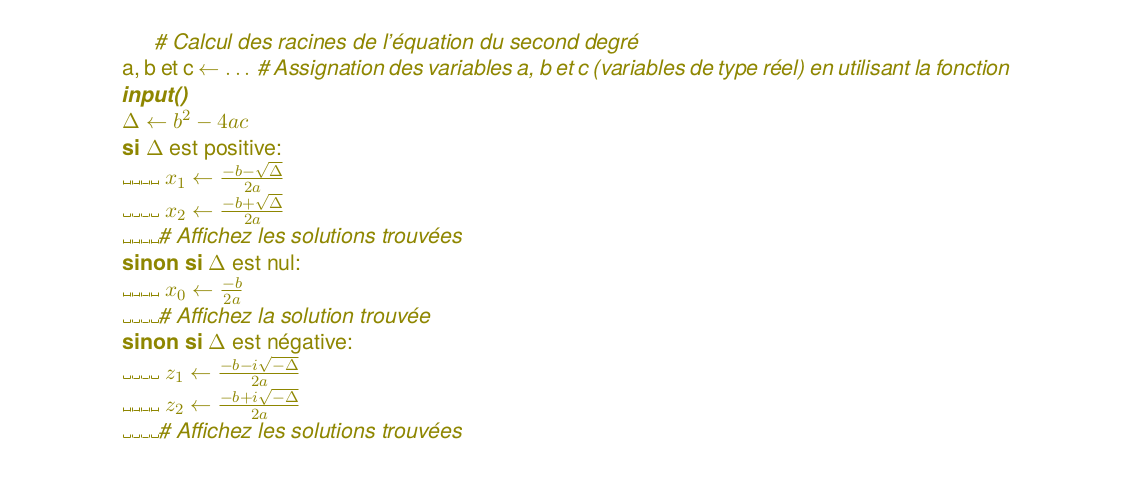
\includegraphics[width=1.2\linewidth]{imgs/algo1.png}}

\vspace{6mm}



% --- end hint in exercise ---


% --- begin solution of exercise ---
\paragraph{Solution.}
\begin{cod}{cbg_gray}\begin{minted}[fontsize=\fontsize{9pt}{9pt},linenos=false,mathescape,baselinestretch=1.0,fontfamily=tt,xleftmargin=2mm]{python}
# %load solution/ex4
"""
Calcul des racines de l'equation du second degré:
a x^2 + b x + c = 0
"""
from math import sqrt

a = float(input("Valeur de a:"))
b = float(input("Valeur de b:"))
c = float(input("Valeur de c:"))

print("L'équation a resoudre est: {} x^2 + {} x + {}".format(a,b,c))

delta = b**2 - 4*a*c  #Calcul du discriminant:

#Resultats des racines suivant la valeur de delta:
if delta > 0:
    x1 = (-b - sqrt(delta))/(2*a)
    x2 = (-b + sqrt(delta))/(2*a)
    # Affichage des solutions trouvées
    print("Les solutions sont réelles: ")
    print("La premiere racine est x1= ",x1)
    print("La seconde racines est x2= ",x2)

elif delta == 0:
    x0 = -b/(2*a)
    # Affichage de la solution trouvée
    print("Il y a une seule solution: ")
    print("La solution est", x0)

elif delta<0:
    z1 = (-b - 1j*sqrt(-delta))/(2*a)
    z2 = (-b + 1j*sqrt(-delta))/(2*a)
    # Affichage des solutions trouvées
    print("Les solutions sont complexes: ")
    print("La premiere racine est z1 = ", z1)
    print("La seconde racine est z2 = ", z2)
\end{minted}
\end{cod}
\noindent

% --- end solution of exercise ---

\subex{b)}
Soit la fonction $f(x) = 0.83 x^2 + 3.8 x + 2.48$. En utilisant le programme précédent, trouvez les solutions pour $f(x) = 0$.


% --- begin solution of exercise ---
\paragraph{Solution.}
Les solutions des $f(x) = 0$ sont réelles:
$x_1 =$ et $x_2 =$

% --- end solution of exercise ---

\subex{c)}
La représentation graphique de $f(x)$ est indiquée ci-dessous:



\vspace{6mm}

% inline figure
\centerline{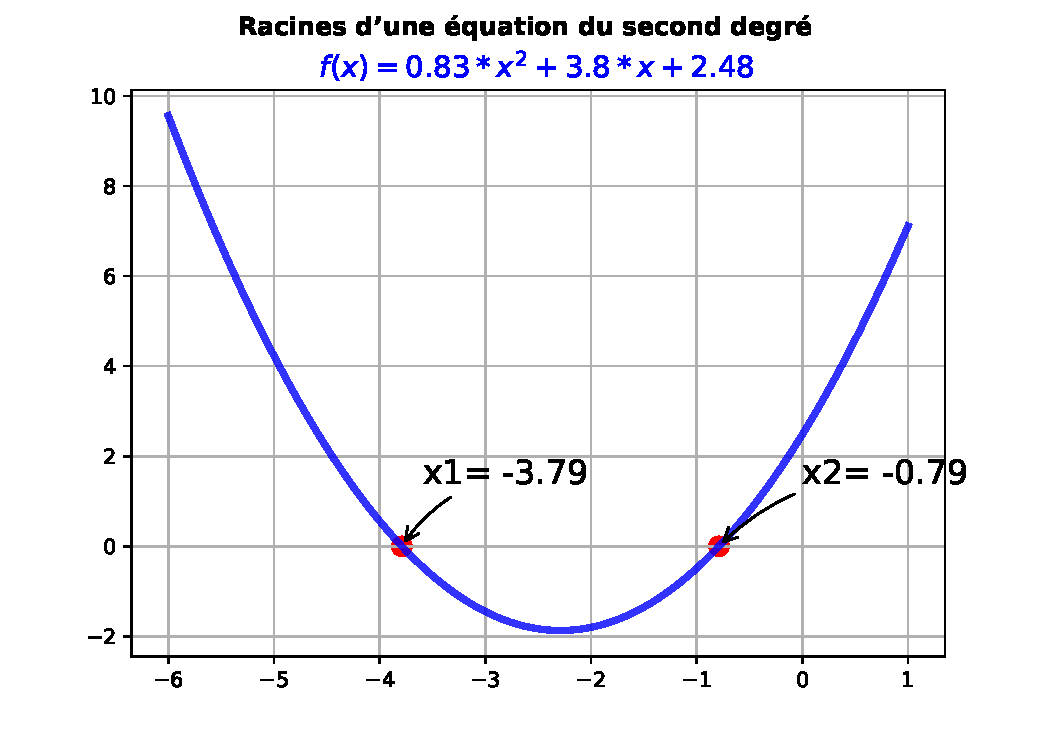
\includegraphics[width=0.9\linewidth]{imgs/ex_fonction1.pdf}}

\vspace{6mm}



Nous allons utiliser une fonction \texttt{EqSecondDegree(a,b,c)} dans \textbf{TD N°3} pour reproduire cette figure en utilisant les bibliothèques \texttt{numpy} et \texttt{matplotlib}.
\begin{itemize}
\item Écrivez la fonction \texttt{EqSecondDegree(a,b,c)} qui \textbf{renvoie} les solutions de l'équation $a x^2 + bx + c = 0$.

\item Enregistrez la fonction \texttt{EqSecondDegree(a,b,c)} dans un script Python \texttt{racines.py}.
\end{itemize}

\noindent
% --- begin solution of exercise ---
\paragraph{Solution.}
\begin{cod}{cbg_gray}\begin{minted}[fontsize=\fontsize{9pt}{9pt},linenos=false,mathescape,baselinestretch=1.0,fontfamily=tt,xleftmargin=2mm]{python}
# %load racines.py
def EqSecondDegree(a,b,c):
    """
    Calcul des racines de l'equation du second degré:
    a x^2 + b x + c = 0
    """
    from math import sqrt

    print("L'équation a resoudre est: {} x^2 + {} x + {}".format(a,b,c))

    delta = b**2 - 4*a*c  #Calcul du discriminant:

    #Resultats des racines suivant la valeur de delta:
    if delta > 0:
        x1 = (-b - sqrt(delta))/(2*a)
        x2 = (-b + sqrt(delta))/(2*a)
        # Affichage des solutions trouvées
        print("Les solutions sont réelles: ")
        print("La premiere racine est x1= ",x1)
        print("La seconde racines est x2= ",x2)
        return x1, x2

    elif delta == 0:
        x0 = -b/(2*a)
        # Affichage de la solution trouvée
        print("Il y a une seule solution: ")
        print("La solution est", x0)
        return x0

    elif delta<0:
        z1 = (-b - 1j*sqrt(-delta))/(2*a)
        z2 = (-b + 1j*sqrt(-delta))/(2*a)
        # Affichage des solutions trouvées
        print("Les solutions sont complexes: ")
        print("La premiere racine est z1 = ", z1)
        print("La seconde racine est z2 = ", z2)
        return z1, z2
\end{minted}
\end{cod}
\noindent

\begin{cod}{cbg_gray}\begin{minted}[fontsize=\fontsize{9pt}{9pt},linenos=false,mathescape,baselinestretch=1.0,fontfamily=tt,xleftmargin=2mm]{python}
# Exécutez le scripte racines.py
EqSecondDegree(a=0.83,b=3.8,c=2.48)
\end{minted}
\end{cod}
\noindent

% --- end solution of exercise ---

\subex{d)}
En utilisant la fonction \texttt{EqSecondDegree(a,b,c)}, trouvez les solutions de $f(x) = 0$.


% --- begin solution of exercise ---
\paragraph{Solution.}
\begin{cod}{cbg_gray}\begin{minted}[fontsize=\fontsize{9pt}{9pt},linenos=false,mathescape,baselinestretch=1.0,fontfamily=tt,xleftmargin=2mm]{python}
from racines import EqSecondDegree
x1, x2 = EqSecondDegree(0.83,3.8,2.48)
print("x1 = {:.3f} et x2 = {:.3f}".format(x1, x2))
\end{minted}
\end{cod}
\noindent

% --- end solution of exercise ---

\end{doconceexercise}
% --- end exercise ---




% --- begin exercise ---
\begin{doconceexercise}
\refstepcounter{doconceexercisecounter}

\exercisesection{Exercise \thedoconceexercisecounter: programmez une boucle \texttt{while} }


Définir une séquence de nombres: $$x_n = n^2 + 1$$

pour les entiers n = 0,1,2,…, N. Écrivez un programme qui affiche $x_n$ pour n = 0,1,…, 20 en utilisant une boucle \texttt{while}.


% --- begin solution of exercise ---
\paragraph{Solution.}
Le programme qui affiche $x_n$ pour n = 0,1,…, 20 en utilisant une boucle \texttt{while} s'écrit:
\begin{cod}{cbg_gray}\begin{minted}[fontsize=\fontsize{9pt}{9pt},linenos=false,mathescape,baselinestretch=1.0,fontfamily=tt,xleftmargin=2mm]{python}
n = 0
while n <= 20:
    x_n = n**2 + 1
    print('x{} = {}'.format(n, x_n))
    n = n + 1
\end{minted}
\end{cod}
\noindent

% --- end solution of exercise ---

\end{doconceexercise}
% --- end exercise ---


% !split


% --- begin exercise ---
\begin{doconceexercise}
\refstepcounter{doconceexercisecounter}

\exercisesection{Exercise \thedoconceexercisecounter: Créer une liste avec une boucle \texttt{while} }


Stockez toutes les valeurs $x_n$ calculées dans l'exercice 5 dans une liste (à l'aide d'une boucle \texttt{while}). Afficher la liste complète (en un seul objet).


% --- begin solution of exercise ---
\paragraph{Solution.}
Les valeurs $x_n$ sont stockés dans une liste \texttt{x} définie:
\begin{cod}{cbg_gray}\begin{minted}[fontsize=\fontsize{9pt}{9pt},linenos=false,mathescape,baselinestretch=1.0,fontfamily=tt,xleftmargin=2mm]{python}
n = 0
x = []  # les x_n valeurs
while n <= 20:
    x.append(n**2 + 1)
    n = n + 1
print(x)
\end{minted}
\end{cod}
\noindent

% --- end solution of exercise ---

\end{doconceexercise}
% --- end exercise ---


% !split


% --- begin exercise ---
\begin{doconceexercise}
\refstepcounter{doconceexercisecounter}

\exercisesection{Exercise \thedoconceexercisecounter: Programmer une boucle \texttt{for} }


Faites l'exercice 6, mais utilisez une boucle \texttt{for}.


% --- begin solution of exercise ---
\paragraph{Solution.}
Le programme avec une boucle \texttt{for} s'écrit:
\begin{cod}{cbg_gray}\begin{minted}[fontsize=\fontsize{9pt}{9pt},linenos=false,mathescape,baselinestretch=1.0,fontfamily=tt,xleftmargin=2mm]{python}
# %load solution/ex7
x = []
for n in range(21):
    x.append(n**2 + 1)
print(x)
\end{minted}
\end{cod}
\noindent
On peut également raccourcir le code en utilisant une liste de compréhension:

\begin{cod}{cbg_gray}\begin{minted}[fontsize=\fontsize{9pt}{9pt},linenos=false,mathescape,baselinestretch=1.0,fontfamily=tt,xleftmargin=2mm]{python}
print([n**2 +1 for n in range(21)])
\end{minted}
\end{cod}
\noindent

% --- end solution of exercise ---

\end{doconceexercise}
% --- end exercise ---


% !split


% --- begin exercise ---
\begin{doconceexercise}
\refstepcounter{doconceexercisecounter}

\exercisesection{Exercise \thedoconceexercisecounter: Ecrire une fonction Python}


Écrivez une fonction \texttt{x(n)} pour calculer un élément dans la séquence $x_n = n^2 + 1 $. Appelez la fonction pour n = 4 et afficher le résultat.


% --- begin solution of exercise ---
\paragraph{Solution.}
La fonction \texttt{x(n)} est définie:
\begin{cod}{cbg_gray}\begin{minted}[fontsize=\fontsize{9pt}{9pt},linenos=false,mathescape,baselinestretch=1.0,fontfamily=tt,xleftmargin=2mm]{python}
def x(n):
    return n**2 +1
print(x(4))
\end{minted}
\end{cod}
\noindent

% --- end solution of exercise ---

\end{doconceexercise}
% --- end exercise ---


% !split


% --- begin exercise ---
\begin{doconceexercise}
\refstepcounter{doconceexercisecounter}

\exercisesection{Exercise \thedoconceexercisecounter: Renvoyer trois valeurs d'une fonction Python}


Écrivez une fonction Python qui évalue les fonctions mathématiques $f(x) = cos(2x)$, $f'(x) = -2sin(2x)$ et $f"(x) = - 4 cos(2x)$. Retourner ces trois valeurs. Écrivez les résultats de ces valeurs pour $x = \pi$.


% --- begin solution of exercise ---
\paragraph{Solution.}
Soit une fonction \texttt{deriv2(x)} qui renvoie les valeurs de $f(x)$, $f'(x)$ et $f"(x)$:
\begin{cod}{cbg_gray}\begin{minted}[fontsize=\fontsize{9pt}{9pt},linenos=false,mathescape,baselinestretch=1.0,fontfamily=tt,xleftmargin=2mm]{python}
from math import sin, cos, pi

def deriv2(x):
    return cos(2*x), -2*sin(2*x), -4*cos(2*x)

f, df, d2f = deriv2(x=pi)

print("f(pi) = {}; df(pi) = {}; d2f(pi) = {} ".format(f, df, d2f))
\end{minted}
\end{cod}
\noindent

% --- end solution of exercise ---

\end{doconceexercise}
% --- end exercise ---


% ------------------- end of main content ---------------

% #ifdef PREAMBLE
\end{document}
% #endif

